\section{Evaluation}
\label{Eva}

In this section, we describle our performance evaluation in simulation and
real-scene experiments. We distribute 130 TI SensorTag sensors in an about
$250~\times~250$ square meters area, with contiki-ng as its operating system. We
use different metrics for various applications and compare our works with other
state-of-the-art works.

\subsection{Routing}

\textbf{Packet recieved ratio.}
Packet recieved ratio is defined as the proportion of the total data packets
recieved by data sink and the the total data packets sent by all nodes, and it
can be formulated as

\begin{equation}
	L = \frac{\sum_{i = 0}^{N}S_i}{R}
\end{equation}

where $L$ reprents the throughput, and $S_i$ and $R$ denotes the number of
packets sent by the $i$-th node and the number of packets recieved by data
sink, respectively.

%\begin{figure}[htbp]
%	\centering
%	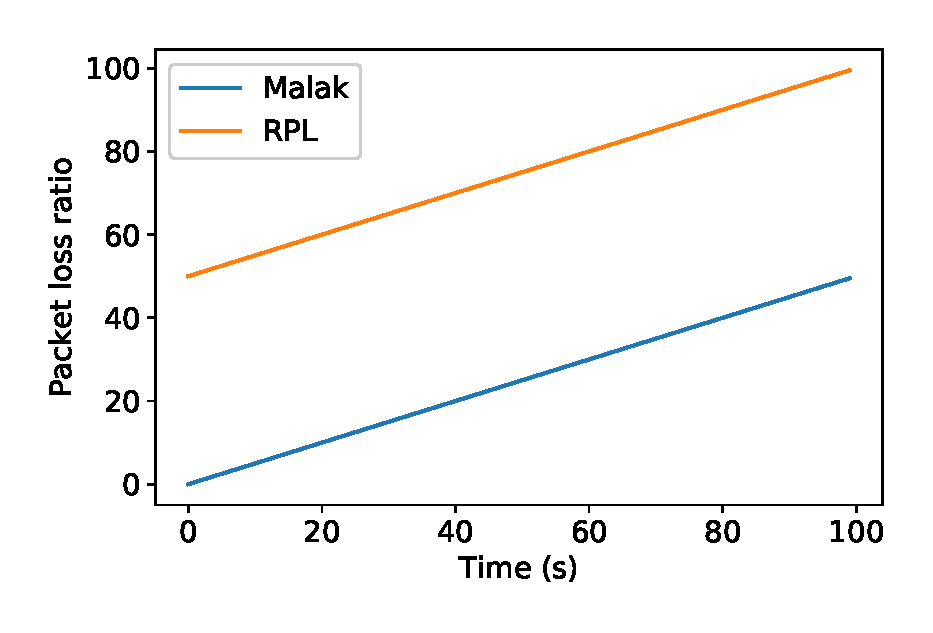
\includegraphics[width=.85\columnwidth]{Figure/packet_loss_ratio}
%	\vspace{-0.1in}
%	\caption{Packet loss ratio in time
%		\textnormal{
%		}}
%	\label{fig:packet_loss_ratio}
%\end{figure}

\begin{figure}[htbp]
	\centering
	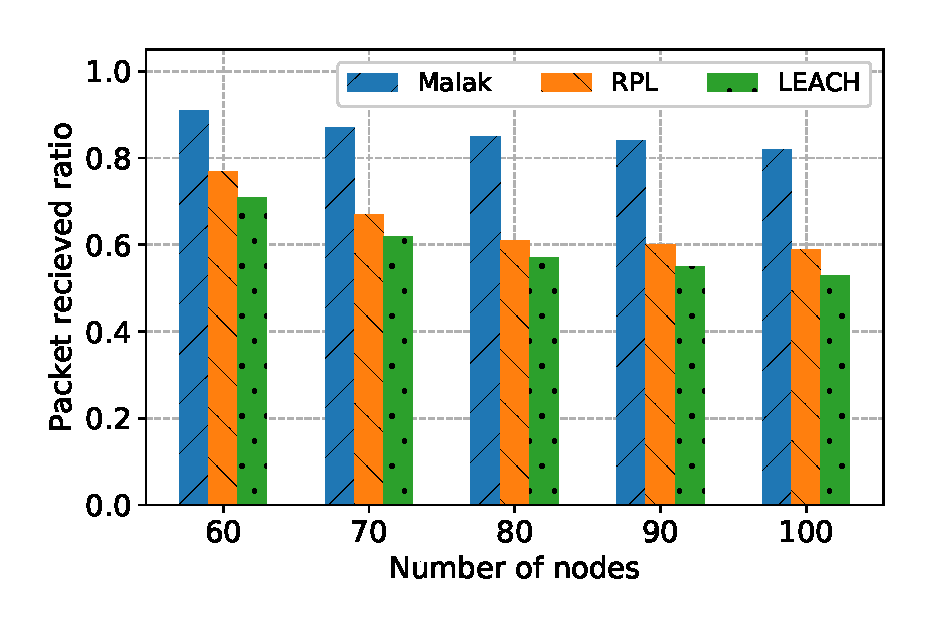
\includegraphics[width=.85\columnwidth]{Figure/packet_loss_ratio_with_size}
	\vspace{-0.1in}
	\caption{Packet recieved ratio
		\textnormal{
		}}
	\label{fig:packet_loss_ratio_with_size}
\end{figure}

Figure~\ref{fig:packet_loss_ratio_with_size} shows two remarkable advantages of
{\sdn}: (1) The packet recieved ratio highly exceeds others'; (2) The decreasing
speed is slow. The reasons are {\sdn} uses UAVs and AI algorithms to help
diagnose and fix routing problems quickly and the cluster mechanism to do local
repair when UAVs are absent.

\textbf{Total throughput.}
Throughput is defined as the the total data packets recieved by data sink, and it
measures the capability and scalability of a network.

\begin{figure}[htbp]
	\centering
	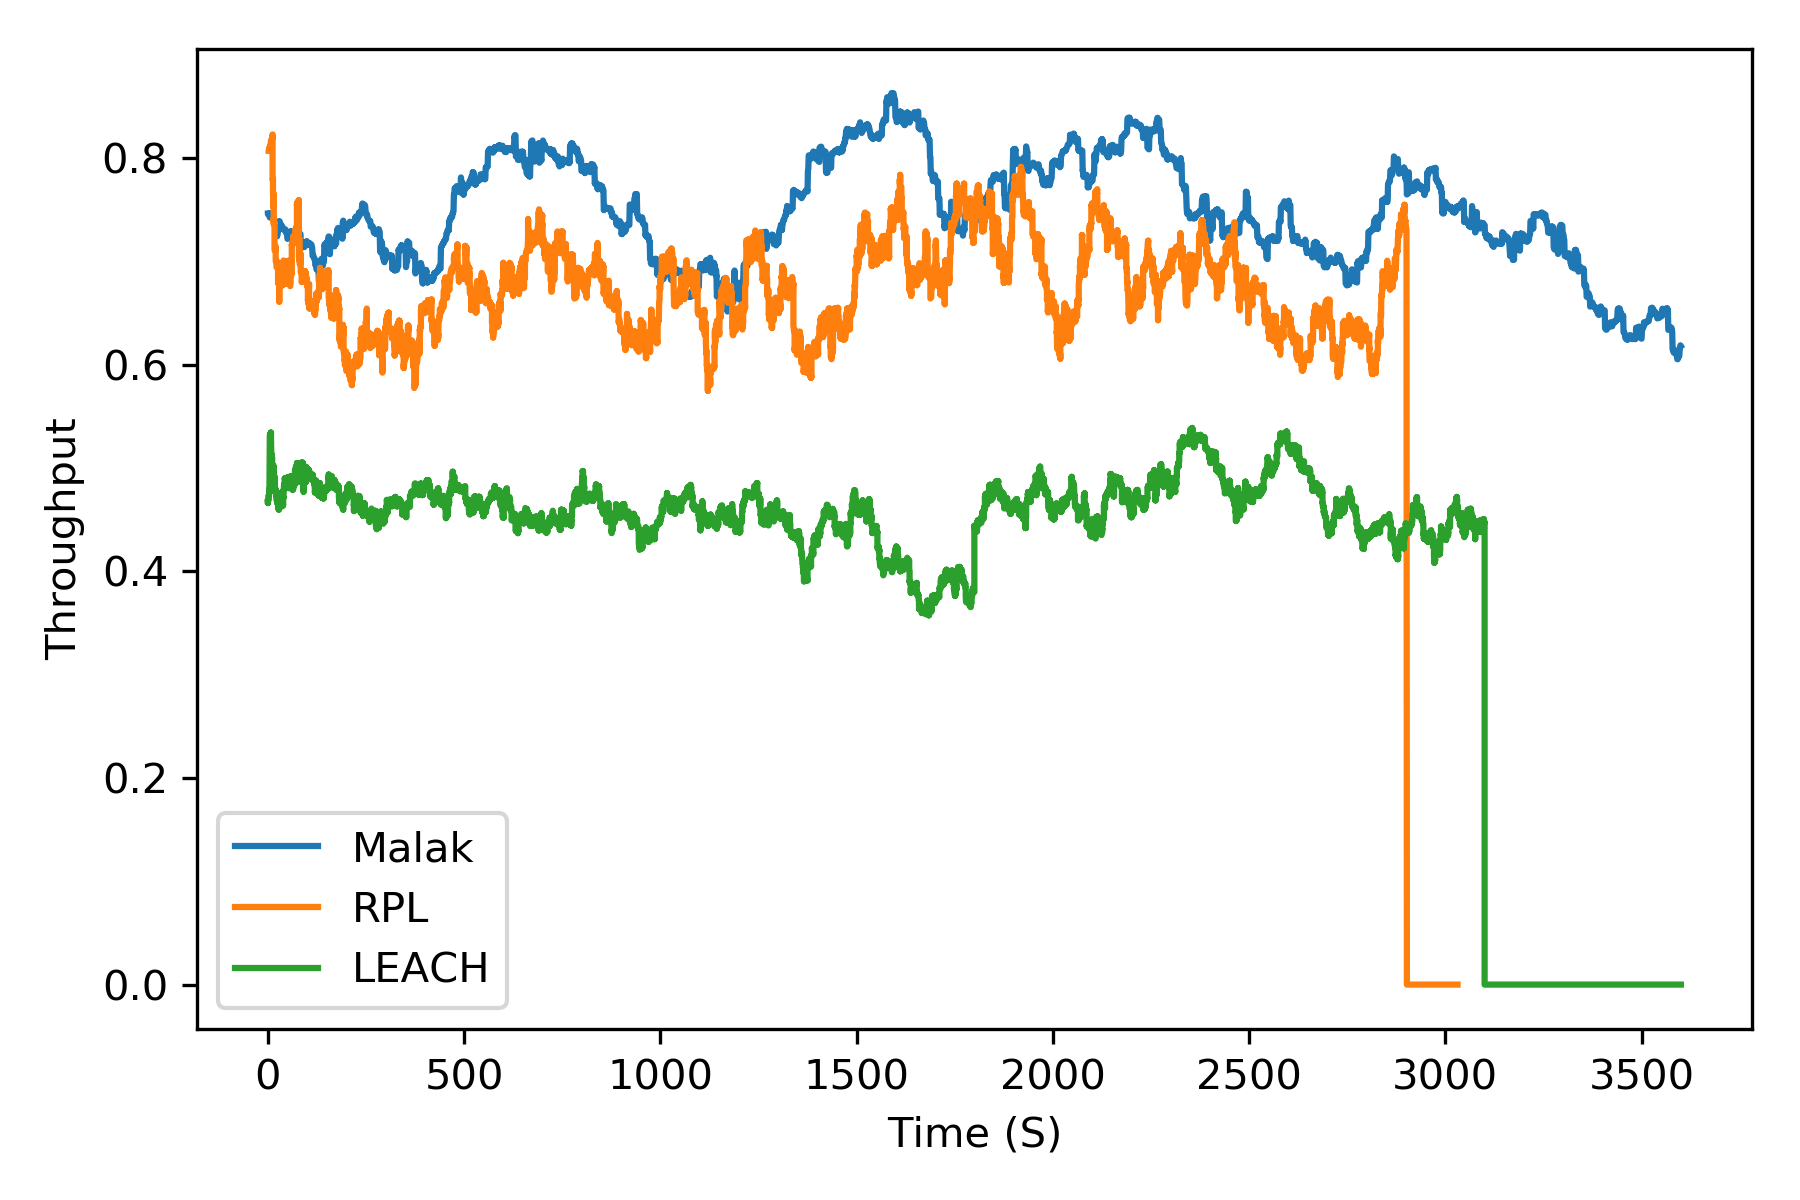
\includegraphics[width=.85\columnwidth]{Figure/throughput}
	\vspace{-0.1in}
	\caption{Routing throughput.
		\textnormal{
			The figure shows throughput corresponding to three kinds of Routing
			algorithms. Throughput can drop to zero when some key nodes are dead
			in the network.
		}}
	\label{fig:throughput}
\end{figure}


Figure~\ref{fig:throughput} compares network throughput by deploying various
routing algorithms. As our {\sdn} uses OSPF, which finds the optimal path from
sensors to data sink, to caculate the route table, its throughput exceeds RPL
and LEACH. Besides, in {\sdn}, sensors' lifetime increases a lot more than
others, because all computation-intensive tasks are done by UAV and sensors do
not need to send packets to negotiate route path, which decrease the energy
consumption with no doubt.

\textbf{Resilience}
Resilience  is a significant metric to evaluate the performance of routing
algorithms. It measures the throughput with various number of node died.
Throughput can drop sharply if a node which most traffic passes by dies and can
be influenced only slightly by death of nodes which no traffic passes through.

We compare the impact caused by death of nodes using throughput between RPL and
{\sdn} and the results are shown in Figure~\ref{fig:fault_tolerance}. Throughput
can be low when the number of death is small, because we distribute the sensors
densely and the collision problem is severe. And the throughput grows as some
node died. But after some key nodes died, the throughput falls down quickly,
however, our {\sdn} still performs better than PRL.

\begin{figure}[htbp]
	\centering
	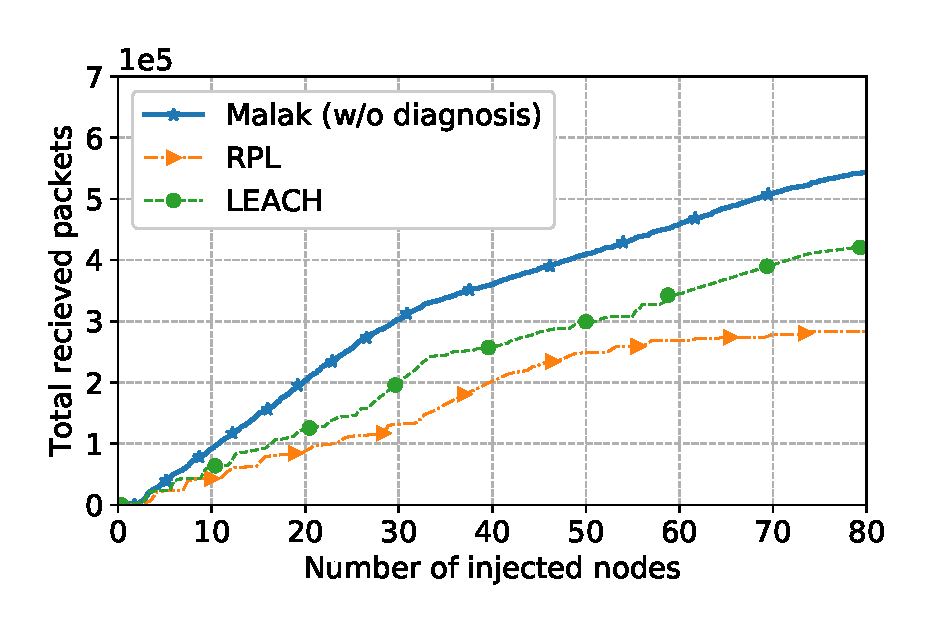
\includegraphics[width=.85\columnwidth]{Figure/fault_tolerance}
	\vspace{-0.1in}
	\caption{Fault tolerance
		\textnormal{
			RPL and {\sdn} are compared on resilience, and {\sdn} perform
			slightly better than PRL.
		}}
	\label{fig:fault_tolerance}
\end{figure}

\textbf{Scalability.}
\begin{figure}[htbp]
	\centering
	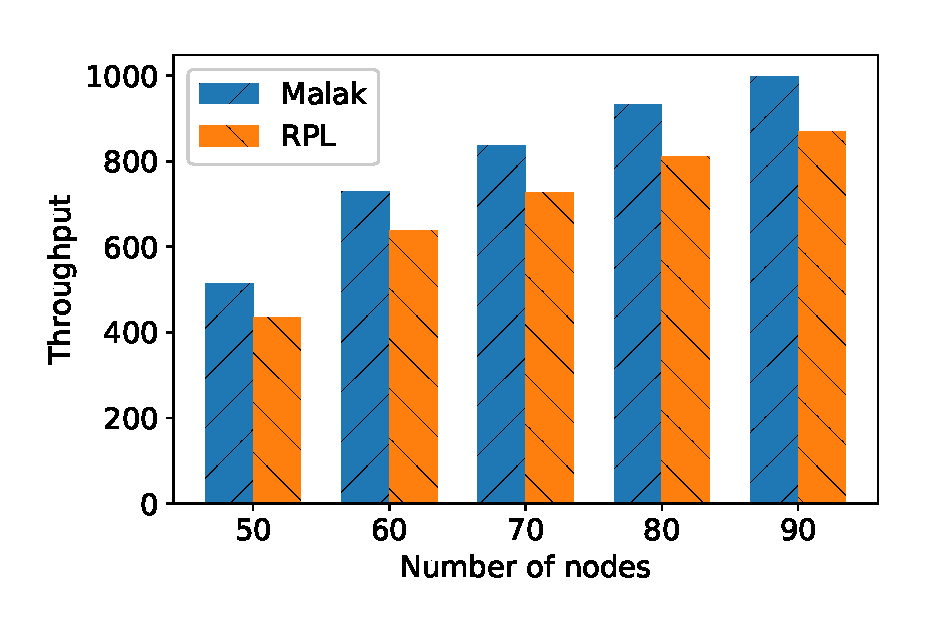
\includegraphics[width=.85\columnwidth]{Figure/scalability}
	\vspace{-0.1in}
	\caption{Scalability
		\textnormal{
			{\sdn} succeeds RPL in different network sizes.
		}}
	\label{fig:scalability}
\end{figure}

\subsection{Network Diagnosis}
\textbf{Failure detection rate.}
Figure~\ref{fig:diagnosis}

\begin{figure}[htbp]
	\centering
	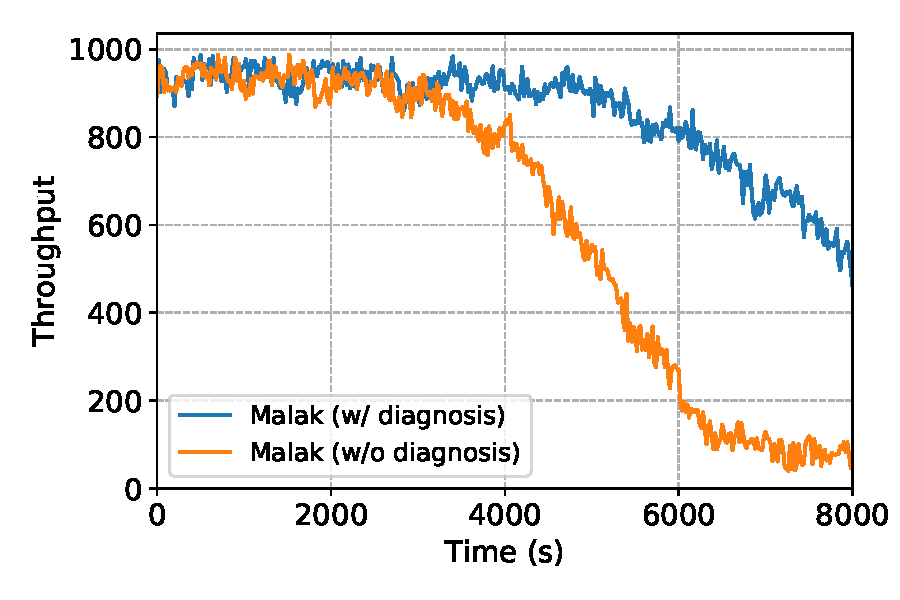
\includegraphics[width=.85\columnwidth]{Figure/diagnosis}
	\vspace{-0.1in}
	\caption{
		\textnormal{
		}}
	\label{fig:diagnosis}
\end{figure}

\begin[htbp]{table}
	\centering
	\begin{tabular}{|c||c|c|c|c|c|}
		\hline
		\diagbox{Type}{Failures} & 1 & 2 & 3 & 4 & 5\\
		\hline
		\hline
		Sensing & 98\% & 95\% & 93\% & 92\% & 90\%\\
		\hline
		Energy & 100\% & 93\% & 92\% & 90\% & 88\%\\
		\hline
		Radio & 100\% & 90\% & 88\% & 84\% & 80\%\\
		\hline
	\end{tabular}
	\caption{Failure detection rate for various failure type and number}
	\label{tab:diagnosis}
\end{table}

\subsection{AI Node Selection}
\textbf{Scalability.}

\subsection{AI Energy Prediction}

We estimate sensor energy consumption by multipling different coefficients on
CPU running time and radio listening and transmitting time and summing them up.
The coefficients are proportional to the working current described in sensor's
DataSheet.

\textbf{Prediction accuracy.}
Figure~\ref{fig:energy_pred:a} shows the real energy consumption curve and the
prediction one.

\begin{figure}[htbp]
	\centering
	\subfloat[Energy prediction]{
		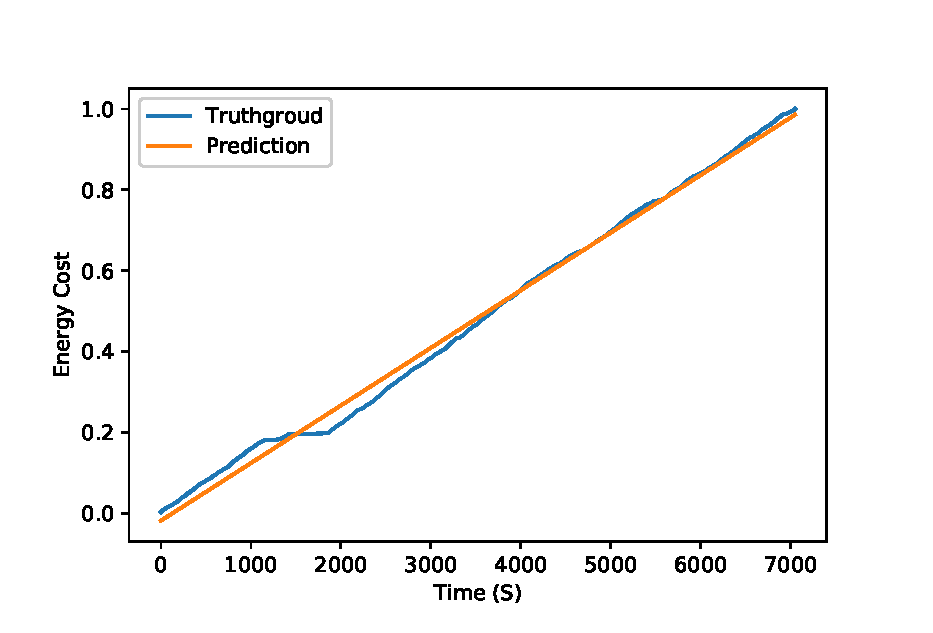
\includegraphics[width=.45\columnwidth]{Figure/energy_pred}
		\label{fig:energy_pred:a}
	}
	\hspace{0.1cm}
	\subfloat[Energy prediction error]{
		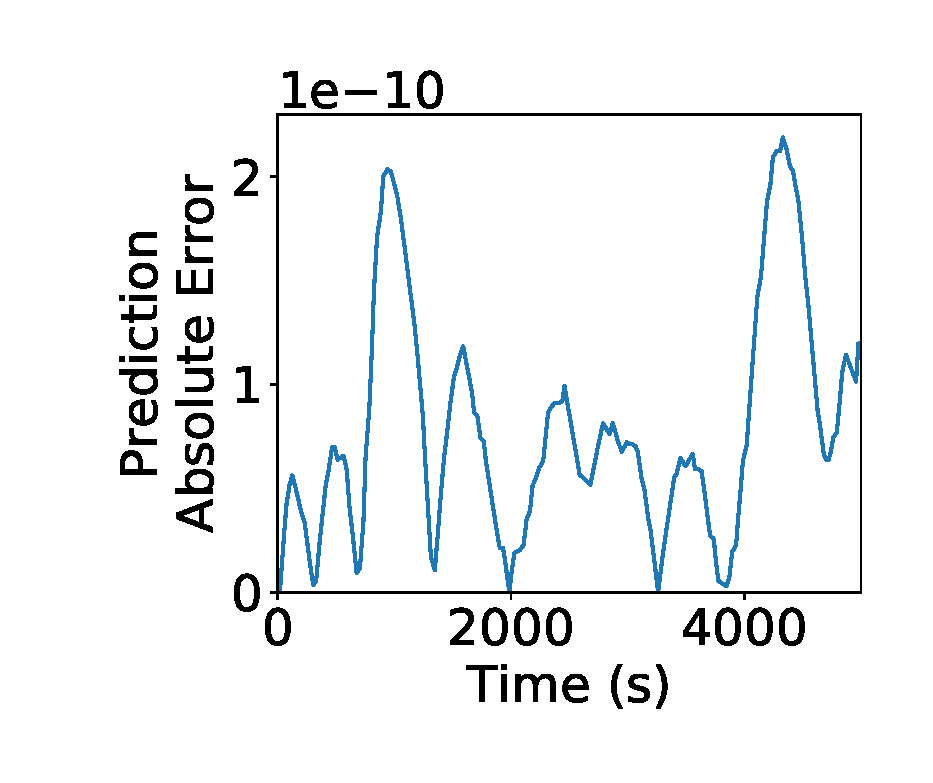
\includegraphics[width=.45\columnwidth]{Figure/energy_pred_err}
		\label{fig:energy_pred:b}
	}
	\vspace{-0.1in}
	\caption{Energy prediction
		\textnormal{
			We use regression method to predict energy consumption and the
			prediction result is consistent with the truthground.  The absolute
			error of energy prediction never exceeds $3\times10^{-10}$ with normalized energy
			(i.e. the maximum energy of a sensor is 1).
		}
	}
	\label{fig:energy_pred}
\end{figure}

\subsection{Multi-tasks}
\textbf{Energy Performance.}

\textbf{Scalability.}
\begin{figure}[htbp]
	\centering
	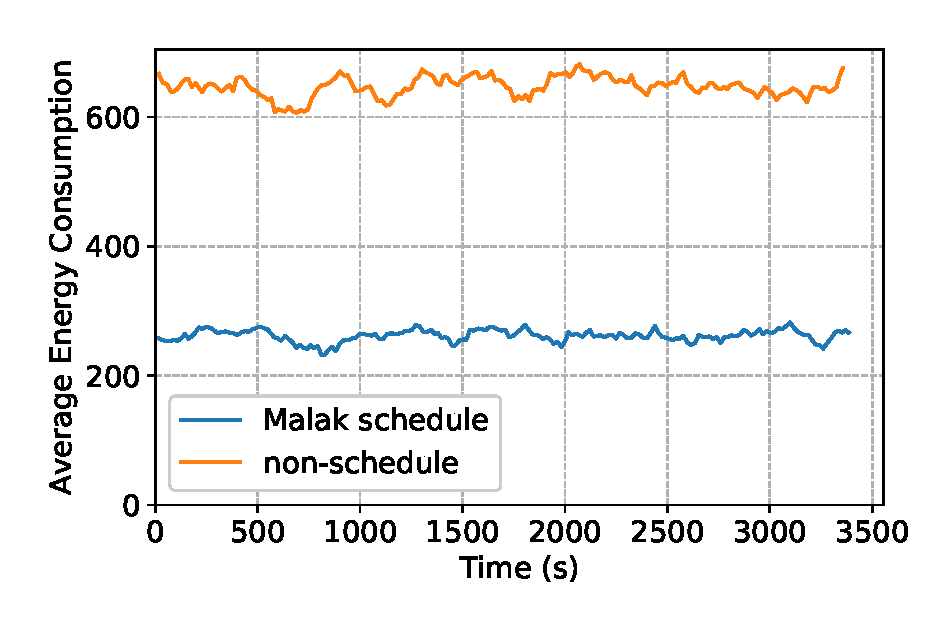
\includegraphics[width=.85\columnwidth]{Figure/multitask_energy}
	\vspace{-0.1in}
	\caption{Average energy consumption with and without multitask schedule
		\textnormal{When with multitask schedule, sensor consumes half of the energy
			comparing to when without multitask schedule.}}
	\label{fig:multitask_energy}
\end{figure}
